\documentclass[letterpaper,11pt]{article}
\setlength{\textwidth}{6.5in}
\setlength{\hoffset}{0in}
%TODO: tweak these a bit more
\setlength{\voffset}{-0.5in}
\setlength{\textheight}{8.75in}
\setlength{\marginparsep}{0in}
\setlength{\marginparwidth}{0in}
\setlength{\oddsidemargin}{0in}

\usepackage{aas_macros}
\usepackage{amssymb}
\usepackage{caption}
\usepackage{hyperref}
\usepackage{listings}
\usepackage{mathabx}
\usepackage{setspace}
\doublespacing
\usepackage[separate-uncertainty, multi-part-units=single]{siunitx}
\DeclareSIUnit\solarradius{R_\Sun}
\DeclareSIUnit\solarmass{M_\Sun}
\usepackage{subcaption}
\usepackage{tabularx}


\usepackage{graphicx}
\usepackage{lineno}
\usepackage[authoryear,square,colon]{natbib}
\bibpunct{[}{]}{;}{a}{,}{,~}

\usepackage{lipsum}

\begin{document}


\title{Searching for the $T^{-3/2}$ Suprathermal Power Law Tail in Parker Solar Probe's IS$\Sun$IS Data}
\author{A. Merrill}
\date{\today}
\maketitle

%\linenumbers

\begin{abstract}
Results from the Advanced Composition Explorer (ACE) and the Ulysses spacecraft suggested the existence of a pervasive power-law spectrum of suprathermal ions in the solar wind with a spectral index of $-{3 \over 2}$.  This distribution is of particular interest to humanity because the suprathermal ions it describes can serve as the seed population for large, destructive events that can harm ground- and air-based equipment.  It has been suggested that various statistical mechanisms can produce the observed spectrum, however the underlying physical phenomena are not yet known.  The spectrum of suprathermal ions is relatively unstudied closer to the Sun than \SI{1}{\astronomicalunit}.  I investigate the first year and a half of Parker Solar Probe's data to find evidence of this spectrum in this previously unstudied region. I find weak evidence to suggest the existence of a common spectrum of protons from 60 to \SI{200}{\kilo\electronvolt} inside the region being studied.  Naive fits to all of the events fail to produce the expected $-{3 \over 2}$, yet some relationship between magnetic turbulence and spectral index is found, as is an apparent relationship between radial distance and spectral index, suggesting some type of asymptotic approach to index $-{3 \over 2}$ as radial distance increases.  Additionally, my results are not incompatible with recent adaptations to some statistical models that yield softer spectra.  Further work is required to uncover the phenomena  in  this  region  that  determine  the  shape  of  the  solar  wind spectrum.
\end{abstract}

\section{Introduction}
\label{sec:intro}
The solar wind in regions above \SI{0.3}{\astronomicalunit} has been studied directly~\citep{McComas2007}, and a considerable understanding of the population of solar wind particles and their distributions has been gained about these regions~\citep{Giacalone2002,McComas2007}.  One particular phenomenon that our current understanding of accelerating processes in the solar wind fails to explain is the existence of a pervasive power law spectrum of solar wind speed with a spectral index of $-5$; alternatively, this can be expressed as a power law of particle energy with spectral index of $-{3 \over 2}$~\citep{Fisk2012}.

%\subsection{Acceleration of Solar Energetic Particles}
%There are at least two signatures seen in solar energetic particle (SEP) events that are seen over a broad spectrum of energies (a few \si{\kilo\electronvolt} to \si{\giga\electronvolt}).  Implusive SEPs can result from magnetic-reconnection driven processes occurring during solar flares.  Gradual SEP events can be created from coronal mass ejection-driven shocks~\citep{Desai2016}.  However, the mechanisms underlying either of these characteristic signatures of the solar wind cannot produce the seemingly omnipresent power-law with index $-{3 \over 2}$.

\subsection{The Seed Population and its Significance}
Observations from ACE show significant differences in the composition of solar energetic particle (SEP) events and solar wind~\citep{Mewaldt2012}.  Additionally, SEPs have been measured to have densities of ${}^3$He and He${}^+$ much greater than thermal solar wind (ie. ${}^3$He is an ion abundant in flares with energy \SI{>10}{\kilo\electronvolt} and He${}^+$ is an interstellar pickup ion), and thus loan themselves to be used as tracers of the source material of the SEP.  Finally, the heavy ion composition of SEP events correlates significantly with background suprathermal densities.  These results suggest that SEPs draw their source material from the suprathermal region~\citep{Desai2006}.  The population of ions in the suprathermal region responsible for the acceleration of SEP events has been coined the \textit{seed population}.

The seed population, having the potential to create large SEP events, is of particular interest to human affairs as these large events can cause significant material and economic damage.  For example, global satellite infrastructure, the electric power grid, and radio communications can be disrupted or destroyed by the effects of large SEP events~\citep{Decadal2013,Desai2016}.  During major magnetic storms induced by large SEP events, atmospheric chemistry at and around the poles can be changed such that significant enhancements in the production and concentration of nitrogen dioxide is observed~\citep{Decadal2013}.  Nitrogen dioxide plays an important role in the equilibrium of ozone maintained in the upper atmosphere, the maintenance of which is crucial in protecting the health of humans on the ground as well as crops and food sources.  Additionally, large SEP events can expose astronauts to many times the safe limits for radiation exposure~\citep{Decadal2013}, creating a problem needing to be addressed before the advent of truly accessible, commercial spaceflight.  Because of the dangerous potential of SEP events, it is a goal of the Committee on a Decadal Strategy for Solar and Space Physics to build an understanding of the creation of these large SEP events so they can be predicted, allowing us to better protect the assets of society.

%Altogether, the seed population is directly concerned with the power law spectrum seen in the solar wind as the seed population for SEP events is composed of suprathermal ions, the amount of which is dictated by the power law spectrum.  I search for the existence of this spectrum of ions in the solar wind in regions below \SI{0.3}{\astronomicalunit}.

\subsection{The Quiet Time Spectrum}
\citet{Fisk2008} propose a model acceleration of the solar wind during quiet times in which particles are accelerated in compressional turbulence which exhibits the observed spectral index of $-{3 \over 2}$.  Quiet times are defined to exclude times of increased particle flux due to acceleration from shocks or large-scale compression regions, while still maintaining sufficient fluxes to observe a spectrum.  In particular, \citet{Fisk2008} use the following model for quiet time events:
\begin{equation}
j = j_0 T^{-{3 \over 2}} \exp(-T / T_0),
\label{eqn:flux}
\end{equation}
where $j_0$ is a normalization constant, $T$ is the energy per nucleon, and $T_0$ is defined as
\begin{equation}
T_0 = \frac{\left \langle \partial u^2 \right \rangle}{r_{g0}}{Q \over A}{r_0 \over u_{sw}}{m_p v_0 \over 2},
\end{equation}
where $r_{g0}$ is the gyroradius of a proton evaluated at speed $v_0$ and location $r_0$, $A$ is the mass number and $Q$ is the charge number, and $m_p$ is the proton mass.

\citet{Schwadron2010} demonstrate how the spectral index $-{3 \over 2}$ could also arise from various different phenomena from those cited in \citet{Fisk2008}.  \citet{Schwadron2010} demonstrate how the superposition of exponential and Gaussian distributions can show power law tails, and subsequently how various phenomena contribute to this.  In particular, \citet{Schwadron2010} show how the same spectral shape can arise from a series Poisson-like processes in which entropy is maximized, a series of Gaussian distributions in which entropy is maximized, or a series of diffusively accelerated particle spectra with individual spectra derived from being subjected to numerous shocks.  \citet{Schwadron2019AGU} elaborates how the superposition of the various processes described in \citet{Schwadron2010} can also result in softer spectra than the pervasive $-{3 \over 2}$.

\subsection{Instrumentation}
Parker Solar Probe (PSP) provides a previously unseen view of the solar wind inside Earth's orbit.  Diving from more than 60 to less than \SI{10}{\solarradius}, the spacecraft plunges into the solar corona to observe the phenomena that accelerate the solar wind and inflate the heliosphere.  PSP's closer view of the Sun can help explain how the corona is heated and how this power law spectrum is created in the solar wind~\citep{McComas2014,McComas2007}.

ACE and Ulysses have performed extensive surveys of the regions at \SI{1}{\astronomicalunit} and between 1 and \SI{\sim 6}{\astronomicalunit}, respectively, that are thus far satisfactory for scientific goals~\citep{McComas2007}.  However, Prior to PSP, our closest equatorial observations of the Sun were performed by the Helios spacecrafts beginning in the late 1970s~\citep{McComas2007}.  Since the launch of the pair of observing spacecraft, particle detector technology has continued to progress.  PSP is equipped with detectors with dramatically increased time and energy resolution, as well as being capable of discerning particle species from the solar wind~\citep{McComas2014}.

I use data from PSP's IS$\Sun$IS EPI-Lo instrument to look for the existence of the common power law tail inside \SI{1}{\astronomicalunit}.  EPI-Lo is a time-of-flight based mass-spectrometer capable of measuring ions and electrons varying from approximately \SI{20}{\kilo\electronvolt} to \SI{5}{\mega\electronvolt}.  Of interest here are EPI-Lo's specific capabilities surrounding protons, for which the instrument is capable of measuring between 0.04 and \SI{7}{\mega\electronvolt}~\citep{McComas2014}.  EPI-Lo is made of eight \SI{45}{\degree} wedge segments, each of which has 10 entrances for particles to strike a solid state detector.  I use EPI-Lo's Channel T data, which is a time-of-flight (ie. SSD not used) total ion channel calibrated assuming only hydrogen.

%\subsection{Layers of Protection for the Earth}
%The planets are protected from galactic cosmic radiation by the ever-flowing solar wind that inflates the heliosphere.  

%The Parker Solar Probe is uniquely positioned to observe the origin of the solar wind.  

\section{Analysis}
\label{sec:analysis}
At the time of beginning the analysis, data from the beginning of PSP's flight (end of September 2019) through early January 2020 were available.  Events were selected by plotting a spectrogram of hourly- and directionally-averaged time-of-flight high energy resolution proton fluxes (Channel T Flux in the IS$\Sun$IS EPI-Lo Level 2 dataproducts) against time and energy for the entire duration of time for which data was available.  Fifteen events were found in PSP's data during this time, the parameters for which can be found in Table \ref{tab:params}.  The spectrogram from which events were selected is shown in Figure \ref{fig:flux_global}.  Increased flux is apparent on a periodic basis occurring approximately every 5 months.  This coincides with solar encounters and has little relation to actual events.

\begin{figure}[htbp]
\centering
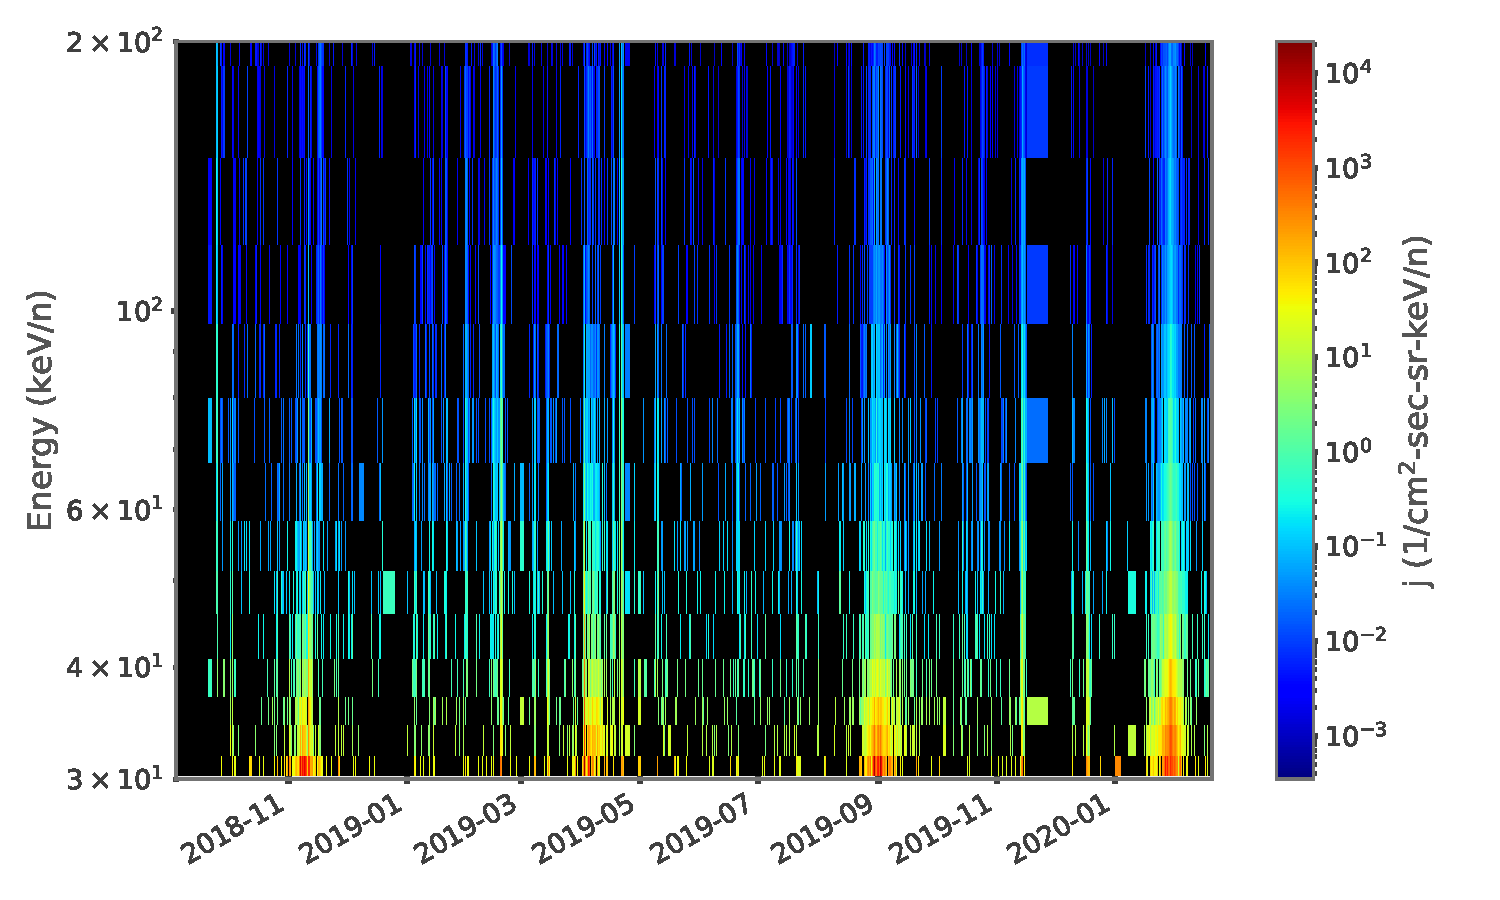
\includegraphics[width=0.9\linewidth]{figures/flux_global.pdf}
\caption{Flux (j) versus energy and time for the duration of the mission at the time data analysis was started.  Individual events generally lasted for the approximate duration of a few days, making them too small to indicate on the spectrogram.  Notice that solar encounters are visible occurring approximately every 5 months starting in November 2018.}
\label{fig:flux_global}
\end{figure}

\begin{table}[htbp]
\resizebox{\textwidth}{!}{
\begin{tabular}{ r c c c c c c }
\\
Event & Start & Stop & Spec. Index & R (\si{\astronomicalunit}) & Peak Flux (\si{n \per \kilo\electronvolt.\centi\meter\squared.\second.\steradian}) & $\eta^2$ \\
\hline
\\
       0 & 2018-09-25 01:54 & 2018-09-25 22:57 & -2.06 & 0.81 &   2.92 & 0.0327 \\ \\
       1 & 2018-11-11 01:39 & 2018-11-12 01:36 & -5.99 & 0.24 &  56.29 & 0.0345 \\ \\
       2 & 2018-11-15 16:33 & 2018-11-19 23:37 & -2.08 & 0.38 &   3.07 & 0.0161 \\ \\
       3 & 2019-01-31 00:21 & 2019-02-01 17:00 & -3.70 & 0.92 &   2.73 &    n/a \\ \\
       4 & 2019-02-13 17:43 & 2019-02-18 00:03 & -3.12 & 0.85 &   2.83 &    n/a \\ \\
       5 & 2019-02-18 05:00 & 2019-02-19 20:55 & -5.06 & 0.83 &  11.68 &    n/a \\ \\
       6 & 2019-03-06 09:17 & 2019-03-08 05:04 & -5.82 & 0.67 &   4.60 & 0.0249 \\ \\
       7 & 2019-03-13 23:33 & 2019-03-15 12:34 & -6.29 & 0.56 &   6.10 & 0.1070 \\ \\
       8 & 2019-04-02 05:44 & 2019-04-03 00:36 & -8.34 & 0.18 & 159.11 & 0.0130 \\ \\
       9 & 2019-04-04 02:36 & 2019-04-04 20:01 & -5.46 & 0.17 &  30.60 & 0.0042 \\ \\
      10 & 2019-04-17 15:36 & 2019-04-18 06:51 & -5.21 & 0.41 &   7.18 &    n/a \\ \\
      11 & 2019-04-20 10:58 & 2019-04-23 19:32 & -3.21 & 0.49 &   5.33 & 0.0112 \\ \\
      12 & 2019-06-19 15:10 & 2019-06-21 22:20 & -3.03 & 0.94 &   1.76 &    n/a \\ \\
      13 & 2019-10-22 11:09 & 2019-10-26 08:04 & -2.62 & 0.88 &   1.67 &    n/a \\ \\
      14 & 2019-11-13 08:30 & 2019-11-16 22:08 & -4.88 & 0.94 &   6.23 &    n/a \\ \\
\hline
\\
\end{tabular}}

\caption{Parameters of the fifteen events identified.  Events for which magnetic field data was unavailable show n/a for $\eta^2$.  Peak flux was determined from the maximum across the entire energy range of EPI-Lo of the average over time and look direction.}
\label{tab:params}
\end{table}

\citet{Fisk2008} suggest a model of compressional acceleration in solar wind turbulence that predicts a functional dependence of flux on energy in the suprathermal tail as shown in Equation \ref{eqn:flux}.  Here, I fit the event spectra to
\begin{equation}
j = \tilde{j_0} T^{\alpha},
\label{eqn:fit}
\end{equation}
where $\tilde{j_0}$ is a normalization constant and $\alpha$ is the spectral index, and both $\tilde{j_0}$ and $\alpha$ are fit parameters.  This simplifies the analysis without loss of validity as parameters included in Equation \ref{eqn:flux} are included in $\tilde{j_0}$.

\subsection{Duration and Directionally Averaged Fits}
The first approach to find evidence of the model in Equation \ref{eqn:fit} fitting the spectra of the events was to simply apply a fit to the data between 40 and \SI{160}{\kilo\electronvolt} of an event-duration- and directionally-averaged spectrum of each event.  This energy region was determined by visual inspection of the events to to fit the region most like a power-law inside the suprathermal region described by \citet{Fisk2008}. This yielded fits like those shown in Figure \ref{fig:naive_fits}.  The exponents of these fits did not match well to the expected $-{3 \over 2}$.

\begin{figure}[htbp]
\centering
\begin{subfigure}{.45\textwidth}
\centering
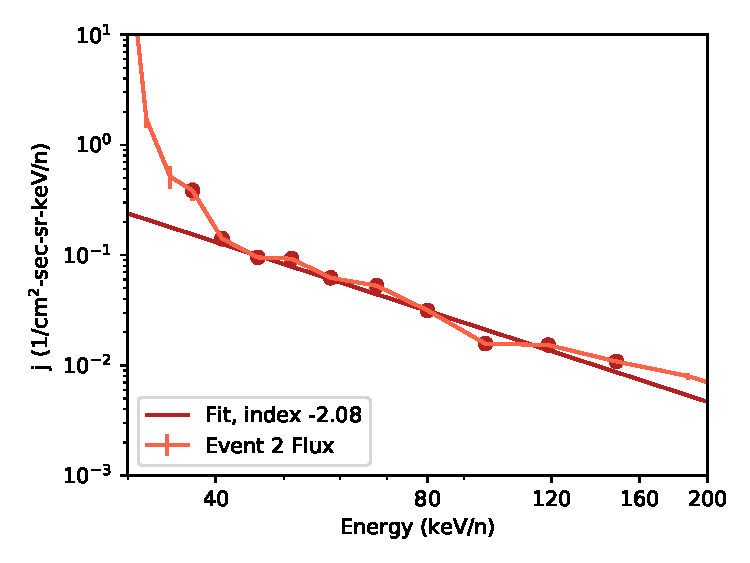
\includegraphics[width=1.\linewidth]{figures/spectrum_02.pdf}
\caption{Event 2}
\end{subfigure}
\begin{subfigure}{.45\textwidth}
\centering
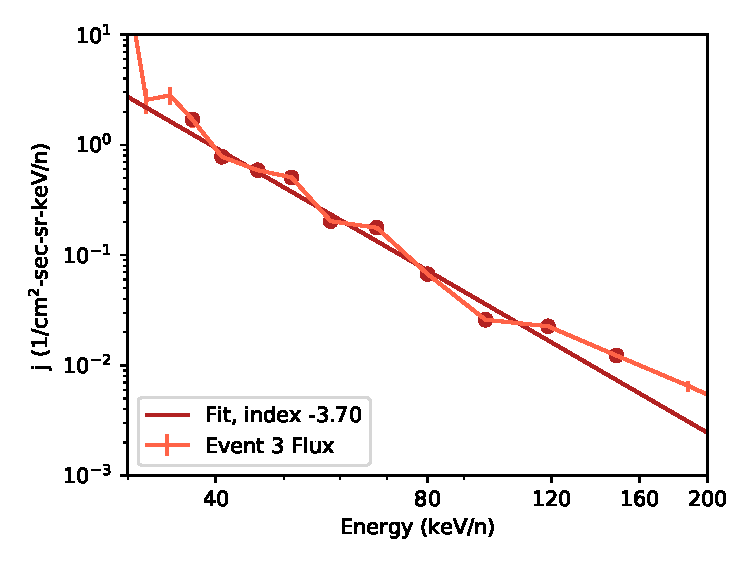
\includegraphics[width=1.\linewidth]{figures/spectrum_03.pdf}
\caption{Event 3}
\end{subfigure}
\caption{Fits of the spectra from Events 2 and  3.  Red points on the spectrum of either plot indicate points used for the fit.}
\label{fig:naive_fits}
\end{figure}

\subsection{Magnitude and Direction of B}
\citet{Fisk2008} note that the common spectrum appears in populations of charged particles subject to non-shock (ie. quiet time) acceleration.  Accordingly, it became necessary distinguish shock and large compressional events from quiet time events.  Analysis by \citet{Cohen2020} and other suggest that the Event 1, shown in Figure \ref{fig:b_rtn_01}, is the result of a CIR.  Work towards identifying the histories of each event in order to classify quiet time from non-quiet time events is in progress.

%I looked at the strength of the three components of the magnetic field relative to eachother over the duration of each event to classify impulsive versus gradual SEP events.  Because the common index is associated only with gradual quiet-time SEP events, it could be necessary to eliminate events that do not fit that criterion from those being considered.  When analyzing the magnetic field a shock appears as a rapid change in the strength and direction of the magnetic field.  Qualitatively representative samples can be seen in Figure \ref{fig:b_rtn}.  Excluding events which were found to have shock-like features in the magnetic field did not yield improved statistics of the remaining spectra and associated fits.

\begin{figure}[htbp]
\centering
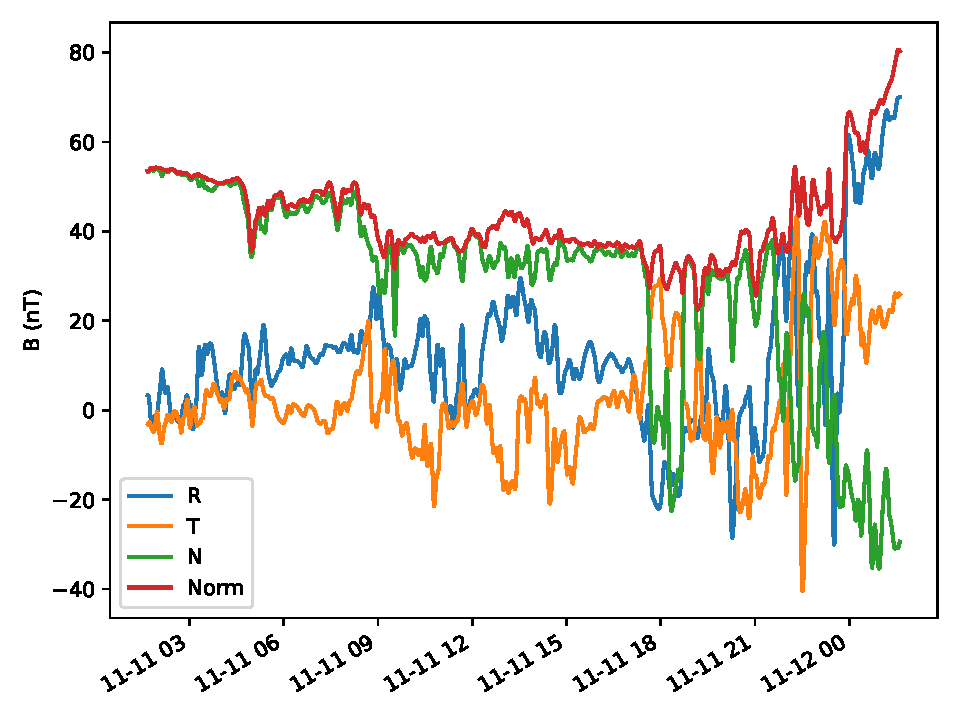
\includegraphics[width=0.75\linewidth]{figures/B_RTN_01.pdf}
\caption{Event 1. Analysis by \citet{Cohen2020} and others suggest this is a CIR.}
\label{fig:b_rtn_01}
\end{figure}

%\begin{figure}[htbp]
%\centering
%\begin{subfigure}{1.\linewidth}
%\centering
%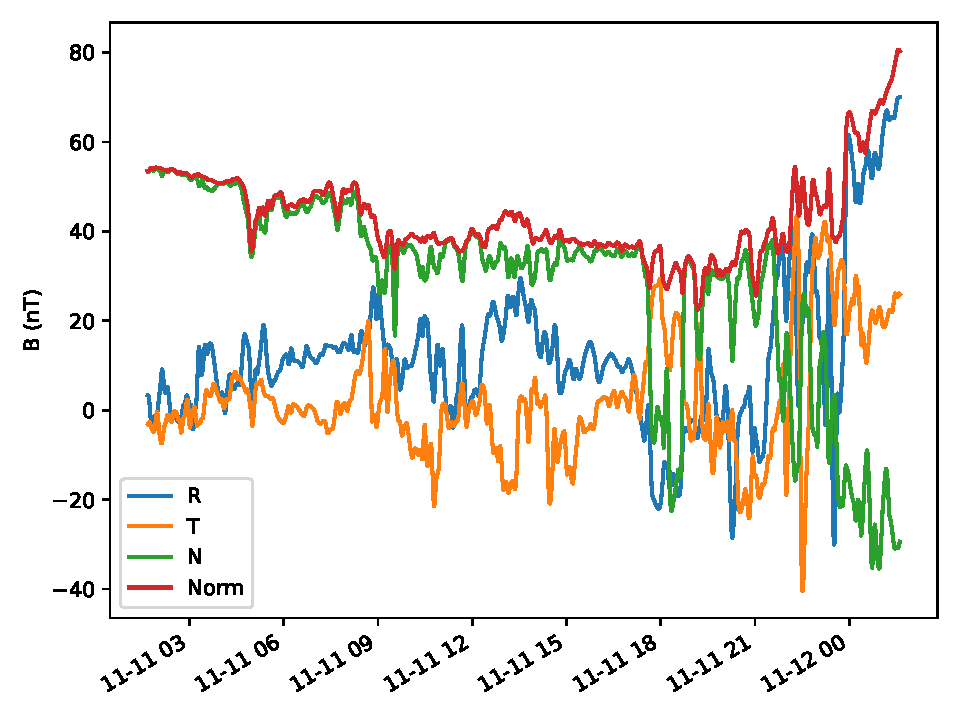
\includegraphics[width=0.75\linewidth]{figures/B_RTN_01.pdf}
%\caption{Event 1. Analysis by \citet{Cohen2020} and others suggest this is a CIR.}
%\label{fig:b_rtn_01}
%\end{subfigure}
%\begin{subfigure}{1.\linewidth}
%\centering
%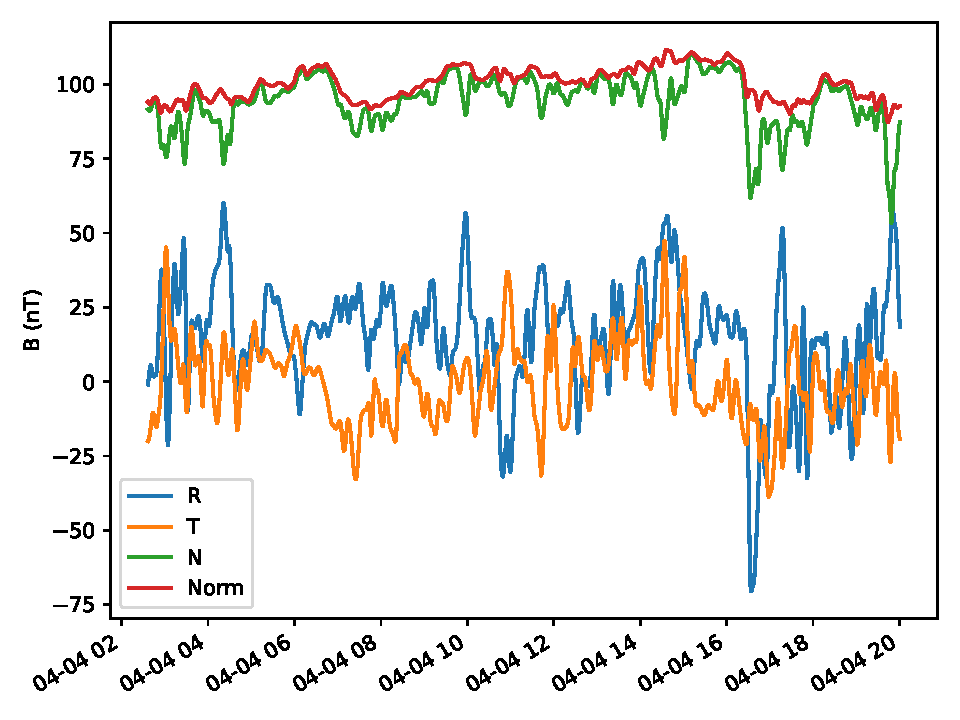
\includegraphics[width=0.75\linewidth]{figures/B_RTN_09.pdf}
%\caption{Event 9.}
%\label{fig:b_rtn_09}
%\end{subfigure}
%\caption{Plots of the three components of B and its magnitude.}
%\label{fig:b_rtn}
%\end{figure}

\subsection{$\eta^2$ and Magnetic Turbulence}
I considered magnetic variance acting as a proxy for magnetic turbulence to indicate accelerating processes in the region of the spacecraft.  \citet{Schwadron1996} suggest the statistical quantity $\eta^2$ to act as a proxy of magnetic turbulence.  Magnetic turbulence indicates the relative strength of acceleration associated with the phenomenon~\citep{Fisk2006}.  Plots of B can be found in Figure \ref{fig:b_rtn_01}, and plots of $\eta^2$ are shown in Figure \ref{fig:etasq}.  An association between magnetic variance and spectrum harness was not found.  However, an apparent upper limit as a function of radius seems to be present in Figure \ref{fig:etasq_daily}.

\begin{figure}[htbp]
\centering
\begin{subfigure}{1.\linewidth}
\centering
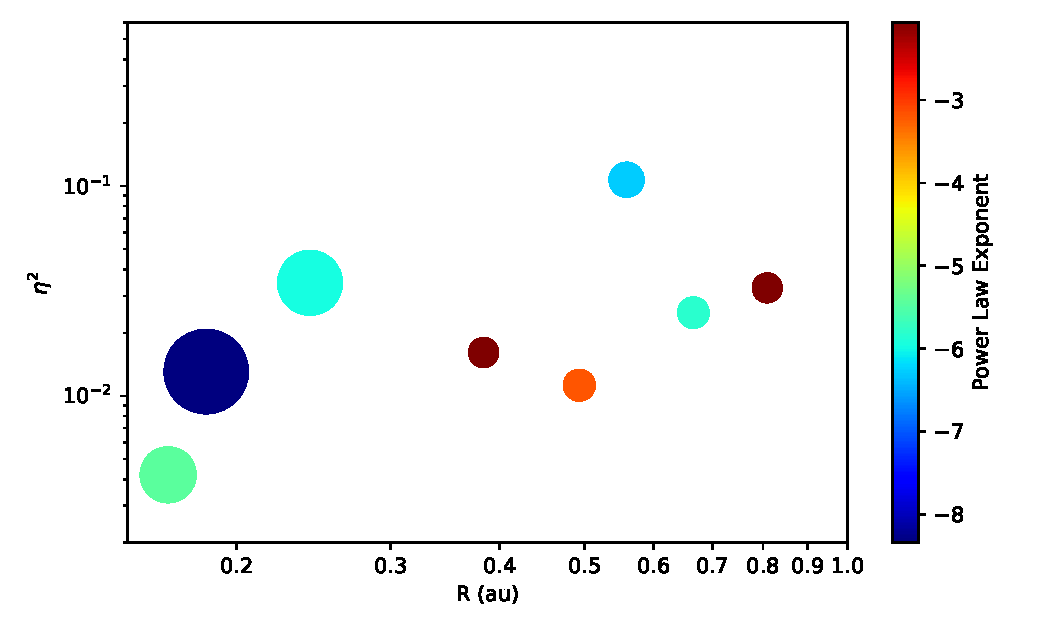
\includegraphics[width=0.9\linewidth]{figures/etasq_vs_R_events.pdf}
\caption{Variance of magnetic field versus radial distance for each event compared with its peak flux and its spectral index.  Size indicates peak flux, color indicates spectrum hardness. \citet{Schwadron1996} propose magnetic variance $\eta^2$ to be a proxy for plasma turbulence.  It appears that a trend exists such that events closer to the sun have less variance in the magnetic field.  Events for which magnetic field data was not available are not shown.}
\label{fig:etasq_events}
\end{subfigure}
\begin{subfigure}{1.\linewidth}
\centering
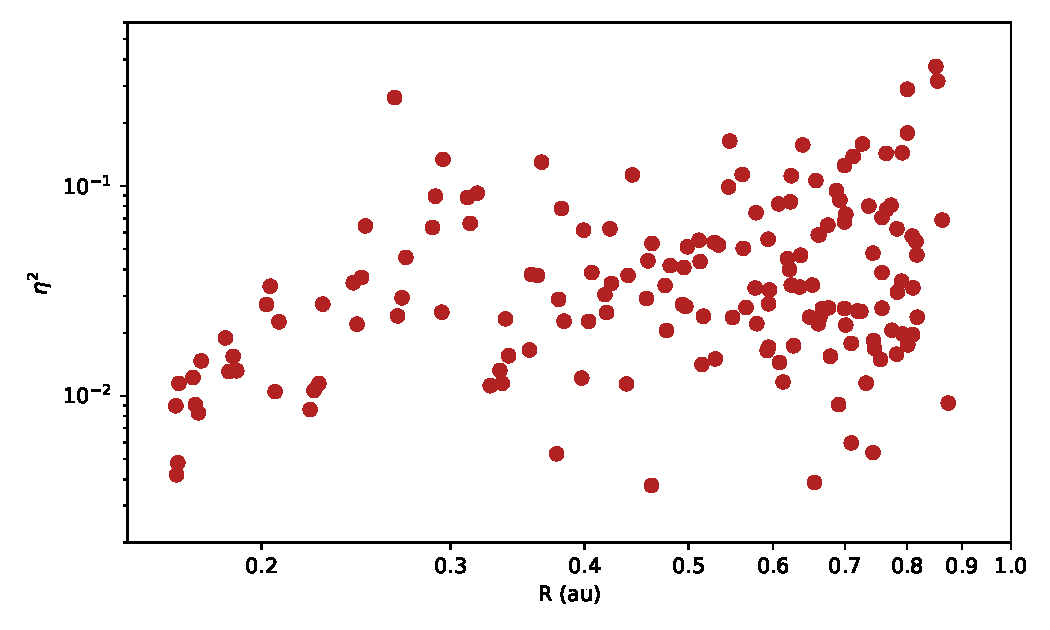
\includegraphics[width=0.9\linewidth]{figures/etasq_vs_R.pdf}
\caption{Variance of magnetic field versus radial distance for each day included in the analysis, (ie. mid September 2018 to January 2020).  The apparent upper limit of magnetic turbulence as a function of radius seen in Figure \ref{fig:etasq_events} is even more apparent here.}
\label{fig:etasq_daily}
\end{subfigure}
\caption{$\eta^2$ versus radial distance.}
\label{fig:etasq}
\end{figure}

\subsection{Spectral Index versus Radius}
I finally considered a relationship between radius and spectral index.  A plot of this data can be seen in Figure \ref{fig:specidx_vs_R}.  An apparent ``spectral hardening'' occurs as radius increases: events appear to have less negative power laws when their flows are observed at greater radii.  Furthermore, this seems to be consistent with the relationship between turbulence and radius observed in Figure \ref{fig:etasq}.  This would suggest that as mechanics in the solar wind drive greater and greater turbulence at larger radii, the spectrum hardens as ions accelerate.

\begin{figure}[htbp]
\centering
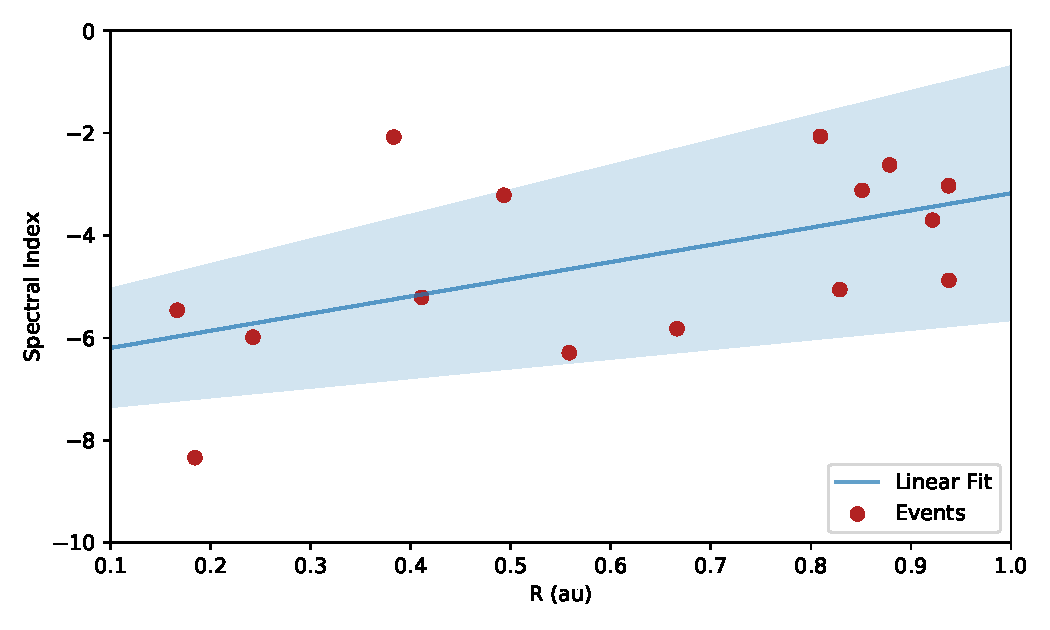
\includegraphics[width=0.9\linewidth]{figures/specidx_vs_R.pdf}
\caption{An apparent relation between radial distance R and the spectral index can be seen in the event data.  Locally this relationship can be modeled by a line, though this is demonstrably not the case at greater radii as the spectral index approaches $-{3 \over 2}$~\citep{Fisk2008,Fisk2006,Schwadron2010,Schwadron2019AGU}.  This fit suggests that spectral index $-{3 \over 2}$ may be approached by an asymptote with respect to radius.  The linear fit between radius and spectral index has slope \SI{3 \pm 1.5}{\per \astronomicalunit} and intercept \SI{-7 \pm 1.0}{}; $r^2 = 0.29$.}
\label{fig:specidx_vs_R}
\end{figure}



\section{Discussion \& Conclusion}
\label{sec:conclusion}
I analyze proton flux data from Parker Solar Probe's first year and a half to find evidence for the common power law tail described in \citet{Fisk2006}.  I do not find evidence to suggest a common spectrum among these data.

None of the fifteen events described in Table \ref{tab:params} have a spectral index near $-{3 \over 2}$.  My analysis is limited in its broad application of fits and its assumption of ``generally'' quiet time conditions.  However, despite that this is the case, with enough events or enough data eventually serendipity would have it that we see an event with the proposed power law tail of $-{3 \over 2}$.

\citet{Schwadron2019AGU} demonstrates how with reasonable assumptions it may be the case the spectral index $-{3 \over 2}$ is the upper limit on spectral hardness for suprathermal ions in the energy range being investigated.  This could serve as an explanation why such a hard spectrum is not observed in the events in the analysis.

The events found here show a clear relationship between spectral hardness and radial distance, as shown in Figure \ref{fig:specidx_vs_R}, despite the poor quality of this fit (ie. $r^2 = 0.29$).  While it cannot be the case that this relationship is linear, the relationship in the domain that is shown suggests that the spectral index of solar wind approaches some value.  Even more interesting is that the hardest \textit{and} softest spectra occur with \SI{0.4}{\astronomicalunit}, suggesting that there may be some mechanism to ``homogenize'' the energy distribution of particles as they flow outward.  This relationship also appears to be compatible with the results shown in Figure \ref{fig:etasq}: greater magnetic turbulence in the solar wind characterizes greater acceleration, increases the spectral hardness~\citep{Fisk2008}.

Also of note is the apparent upper limit as a function of radial distance on magnetic turbulence as quantified by $\eta^2$.  This is shown in Figure \ref{fig:etasq}.

Altogether, I consider here a naive approach without disregarding any event that may include processes originally excluded in \citet{Fisk2008}.  I search for a relation of spectral index with magnetic turbulence, quantified by $\eta^2$, and radial distance.  I fail to find evidence suggesting the existence of a common spectral of suprathermal ions in the region \SI{<1.}{\astronomicalunit}.  However, I find significant evidence to suggest some relationship between radial distance and spectral index and radial distance and an upper limit on magnetic turbulence.



\section{Future Work}
\label{sec:future}
Some extensions to this study could include the following:

\begin{itemize}
\item Analysis on a moving average of each event may show different results or evidence of the common spectrum.  This would additionally benefit from being able to compare a moving average of the spectrum and its index to radius as well.
\item Compare events with other authors and observatories and exclude events on this basis, such as \citet{Cohen2020}.
\end{itemize}



\section{Acknowledgments}
The author wishes to sincerely thank Dr. Jonathan Niehof and Professor Nathan Schwadron for sharing their expertise and guidance throughout the research process, without which this work could not have been accomplished. In addition, the author would like to thank Dr. Dana Filoti and Professor James Ryan for their feedback during the University of New Hampshire Undergraduate Research Conference in Physics.

\bigskip

\noindent This work was supported by NASA Prime Contract No. 136435.



\bibliographystyle{thesis}
%\bibliographystyle{abbrv}
%\bibliographystyle{plainnat}
\bibliography{thesis}

\end{document}
